\section{Specific Requirements}
Text
\subsection{External interface requirements}
Text
\subsubsection{User interfaces}

\begin{figure}[h!]
    \centering
    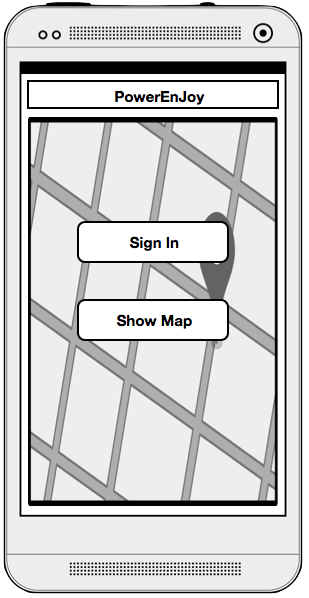
\includegraphics[scale=0.3]{1FirstScreen.png}
    \label{fig:1FirstScreen}
    \\From the first screen a user can either sign in, or create a new account if he is a new user, or consult the map of available Cars.
\end{figure}

\begin{figure}[h!]
    \centering
    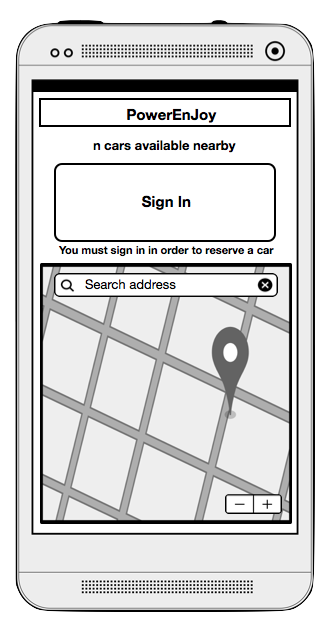
\includegraphics[scale=0.3]{2MapNotLogged.png}
    \label{fig:2MapNotLogged}
    \\If a user chooses the map, he will see a map with all the available cars and he will be asked to sign in in order to proceed with the reservation.
\end{figure}

\begin{figure}[p!]
    \centering
    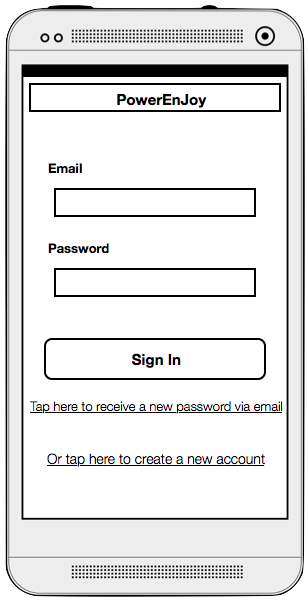
\includegraphics[scale=0.3]{3LoginForm.png}
    \label{fig:3LoginForm}
    \\Whether a user started from the map or from the first screen, he will have to either enter his credential or register. In case of forgotten credential he is given the possibility to ask for a new password too.
\end{figure}

\begin{figure}[p!]
    \centering
    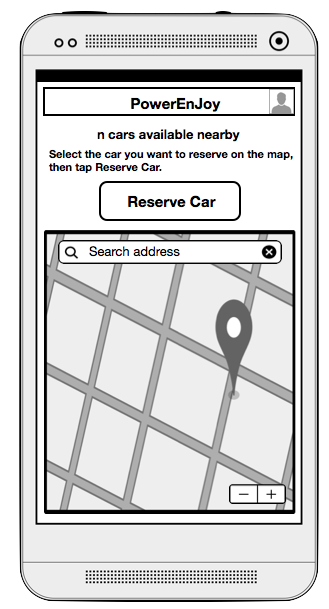
\includegraphics[scale=0.3]{4CarReservationA}
    \label{fig:4CarReservationA}
    \\A PowerUser can look for a suitable Car nearby his position, or entering an adress in the appropriate bar above the map. After finding a Car the PowerUser can reserve it.
\end{figure}

\begin{figure}[p!]
    \centering
    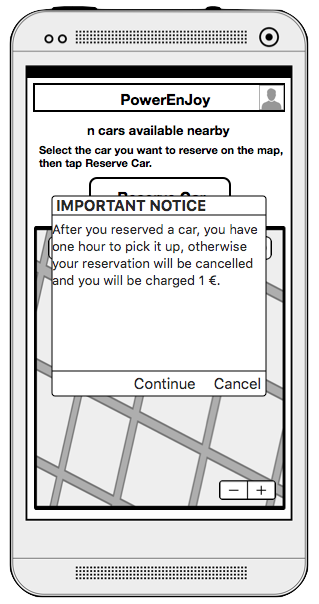
\includegraphics[scale=0.4]{4CarReservationB.png}
    \label{fig:4CarReservationB}
    \\Before actually reserving a Car, the system reminds the PowerUser about the one hour expiration of his reservation and the relative penalty fee.
\end{figure}

\begin{figure}[p!]
    \centering
    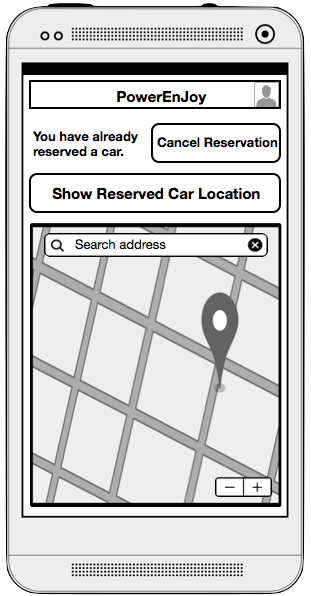
\includegraphics[scale=0.3]{5CarReserved.png}
    \label{fig:5CarReserved}
    \\The selected Car has been reserved. Now a PowerUser can cancel his reservation or look for his car thanks to the provided map.
\end{figure}

\begin{figure}[p!]
    \centering
    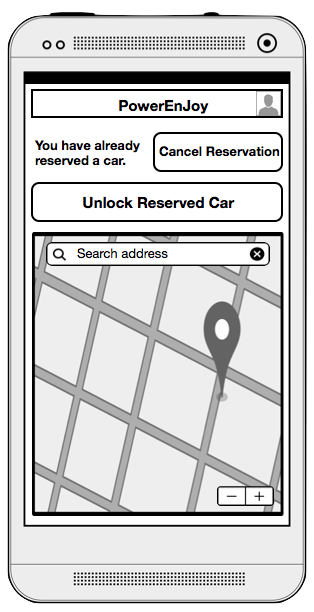
\includegraphics[scale=0.3]{6CarNearby.png}
    \label{fig:6CarNearby}
    \\When a PowerUser is near his reserved Car, he is given the possibility to ask the system to unlock it. If the PowerUser changes his mind he can still cancel the reservation, this possibility will remain valid until the PowerUser ignites the engine. 
\end{figure}

\begin{figure}[p!]
    \centering
    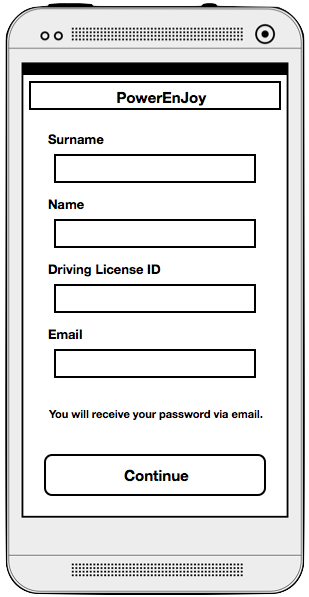
\includegraphics[scale=0.3]{7RegistrationFormA.png}
    \label{fig:7RegistrationFormAForm}
    \\This is the first page that requires a new user to enter his personal data.
\end{figure}

\begin{figure}[p!]
    \centering
    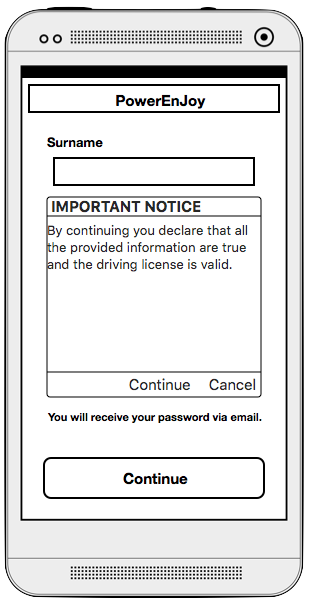
\includegraphics[scale=0.3]{7RegistrationFormB.png}
    \label{fig:7RegistrationFormB}
    \\In order to stress the importance for the user to enter real and correct data, the system reminds the user about this.
\end{figure}

\begin{figure}[p!]
    \centering
    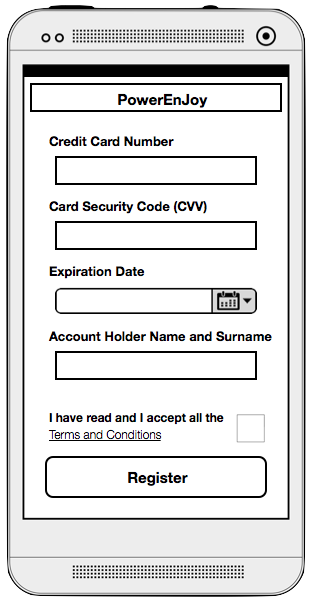
\includegraphics[scale=0.3]{7RegistrationFormC.png}
    \label{fig:7RegistrationFormCnForm}
    \\Last page of the registration form, the user is asked for his payment information. Furthermore he will have to accept the terms and conditions of the service in order to complete the registration.
\end{figure}

\begin{figure}[p!]
    \centering
    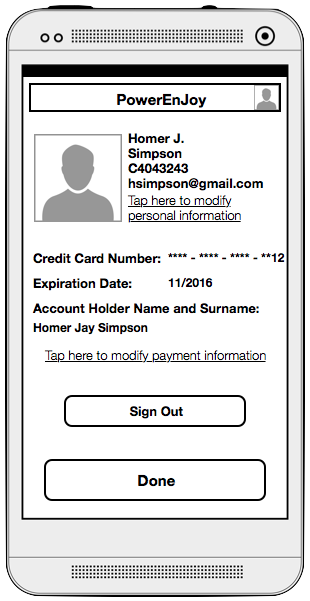
\includegraphics[scale=0.3]{8PersonalAccountPage.png}
    \label{fig:8PersonalAccountPage}
    \\A PowerUser can access his personal account page by tapping on the avatar in the up right corner of his screen. By doing so, this is what he will be shown. From this page it is also possible to modify both personal and payment information.
\end{figure}

\begin{figure}[p!]
    \centering
    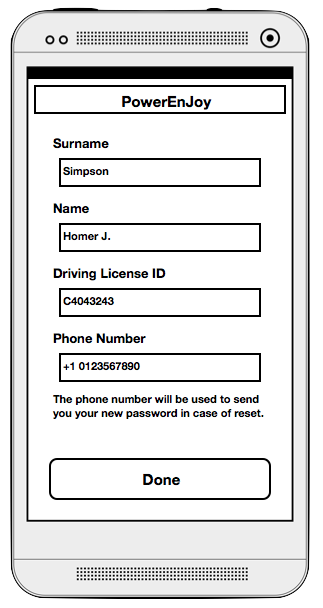
\includegraphics[scale=0.3]{9PersonalDataModification.png}
    \label{fig:9PersonalDataModification}
    \\This is the page to be used by a PowerUser in order to modify his personal information.
\end{figure}

\begin{figure}[h!]
    \centering
    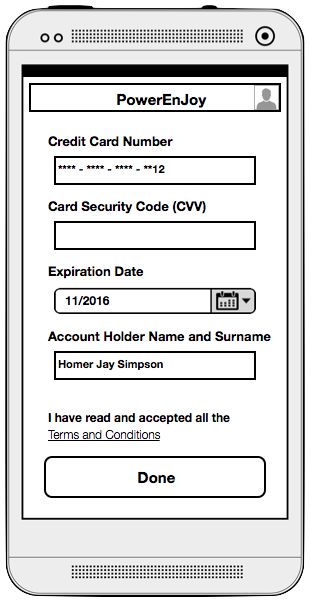
\includegraphics[scale=0.3]{10PaymentSystemDataModification.png}
    \label{fig:10PaymentSystemDataModificationForm}
    \\This is the page to be used by a PowerUser in order to modify his payment information.
\end{figure}

\subsubsection{Hardware interfaces}
Text
\subsubsection{Communication interfaces}
Text
\subsubsection{Software interfaces}
Text
\subsection{Functional requirements}
\begin{itemize}
\item At least a free parking slot is available for the user among all Safe Areas.
\item Special Parking Areas provide at least N\# power sockets as exclusively available to PowerEnJoy customers.
\item No Car with less than B\% battery charge is taken into account while giving to the user a set of available for booking Cars.
\item No Car that is currently under charging and has less than C\% battery charge is taken into account while giving to the user a set of available for booking Cars.
\end{itemize}
\subsection{Use cases}
Text